\documentclass[11pt]{standalone}

\usepackage{helvet}
\usepackage{units}
\usepackage{textcomp}

\usepackage{ifthen}
\usepackage{tikz} 
\usetikzlibrary{shapes.misc}
\usetikzlibrary{arrows,arrows.meta}
\usetikzlibrary{calc,intersections, patterns, math}
\usetikzlibrary{decorations.pathmorphing}
\usetikzlibrary{shapes.geometric}

\definecolor{pfeil}{RGB}{168,167,167}
\definecolor{petrol}{RGB}{0, 118, 136}
\definecolor{blue}{RGB}{0, 118, 136}
\definecolor{white}{RGB}{35,35,35}
% \definecolor{blue}{RGB}{100, 100, 255}
\definecolor{darkgoldenrod}{RGB}{184, 134, 11}
\colorlet{petrol-lighter}{petrol!40}
\colorlet{darkgoldenrod-lighter}{darkgoldenrod!40}
\definecolor{background}{RGB}{35,35,35}

\begin{document}

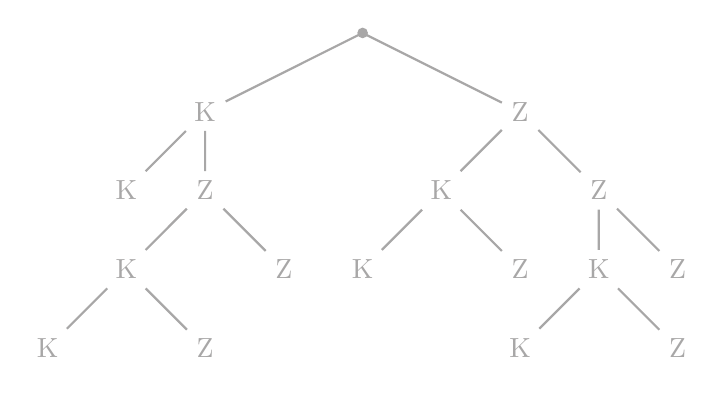
\begin{tikzpicture}[pfeil,yscale=-1]
	\draw[fill] (0,0) coordinate (S) circle (0.06);
	\node[name=K1] at (-2,1) {K};
	\node[name=Z1] at (2,1) {Z};
	\draw[thick] (S) -- (K1) (S) -- (Z1);
	\node[name=K2] at (-3,2) {K};
	\node[name=Z2] at (-2,2) {Z};
	\draw[thick] (K1) -- (K2) (K1) -- (Z2);
	\node[name=K3] at (1,2) {K};
	\node[name=Z3] at (3,2) {Z};
	\draw[thick] (Z1) -- (K3) (Z1) -- (Z3);
	\node[name=K4] at (-3,3) {K};
	\node[name=Z4] at (-1,3) {Z};
	\draw[thick] (Z2) -- (K4) (Z2) -- (Z4);
	\node[name=K5] at (0,3) {K};
	\node[name=Z5] at (2,3) {Z};
	\draw[thick] (K3) -- (K5) (K3) -- (Z5);
	\node[name=K6] at (3,3) {K};
	\node[name=Z6] at (4,3) {Z};
	\draw[thick] (Z3) -- (K6) (Z3) -- (Z6);
	\node[name=K7] at (-4,4) {K};
	\node[name=Z7] at (-2,4) {Z};
	\draw[thick] (K4) -- (K7) (K4) -- (Z7);
	\node[name=K8] at (2,4) {K};
	\node[name=Z8] at (4,4) {Z};
	\draw[thick] (K6) -- (K8) (K6) -- (Z8);
\end{tikzpicture}




\end{document}
